The detailed information of programming are listed in Table.\ref{tab:environment}.
\begin{table}[!hpbt]
	\centering
	\begin{tabular}{ll}
	\hline
	\multicolumn{1}{|l|}{Attribute} & \multicolumn{1}{|l|}{Content}  \\ \hline
	\multicolumn{1}{|l|}{Operation System}                     & \multicolumn{1}{|l|}{\textbf{Windows SDK edition: 10.0}}  \\ \hline
	\multicolumn{1}{|l|}{Integrated Development Environment}      & \multicolumn{1}{|l|}{\textbf{Visual Studio 2019(v142)}}    \\ \hline
	\multicolumn{1}{|l|}{Solution Settings}                       & \multicolumn{1}{|l|}{\textbf{Release in x86 Platform}}\\\hline
	\multicolumn{1}{|l|}{Optimization}  & \multicolumn{1}{|l|}{\textbf{O2 optimize}} \\ \hline
	\multicolumn{1}{|l|}{Programming Language} & \multicolumn{1}{|l|}{\textbf{C\#}} \\ \hline
	\multicolumn{1}{|l|}{Framework} & \multicolumn{1}{|l|}{\textbf{. Net framework 4.7.2}}\\ \hline
	\multicolumn{1}{|l|}{Source Code hosting Platform} & \multicolumn{1}{|l|}{\textbf{Github}} \\ \hline
	\end{tabular}
	\caption{Settings and Attribute}
	\label{tab:environment}
\end{table}

In order to make the operation more smooth, all the program environment and settings are completed and included in the file package. Just required to follow the steps below to run the program.
\begin{enumerate}
\item Open the package and find the Information System Project.exe file. Double-click the file to enter the program interface as Figure.\ref{fig:init} exactly.
\begin{figure}[!htbp]
	\centering
	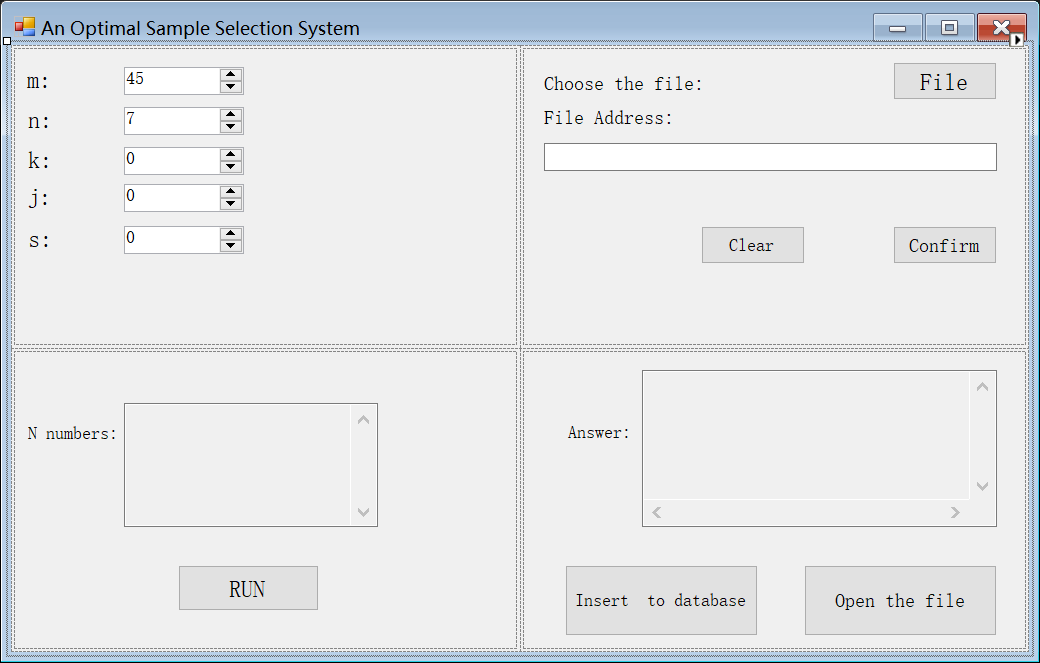
\includegraphics[width=0.75\textwidth]{images/initial.png}
	\caption{Initial GUI}
	\label{fig:init}
\end{figure}

In order to record the relevant output data of the program and facilitate display and modification later. It is required to create a \emph{.mdb} file to store it, which is called ---.mdb in project package.

\item Choose the data of each parameter and input on the program surface as Figure.\ref{fig:st1}.
\begin{figure}[!htbp]
	\centering
	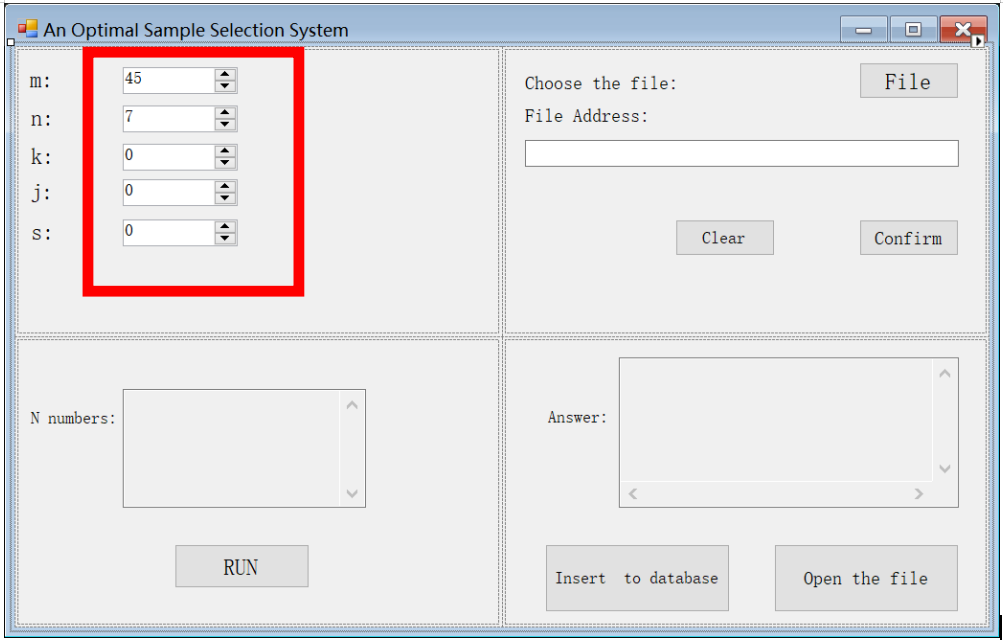
\includegraphics[width=0.75\textwidth]{images/step1.png}
	\caption{Step1}
	\label{fig:st1}
\end{figure}

\item Choose the DB file to store and operate the data, click the button \textbf{File} and choose the \emph{.mdb} as Figure.\ref{fig:st2}
In the previous step and \textbf{Confirm} if all get right.(\textbf{Clear}\textit{ is a function that clear all the data you have input, 
including the parameter followed \textup{Figure.\ref{fig:st3}}})
\begin{figure}[!htbp]
	\centering
	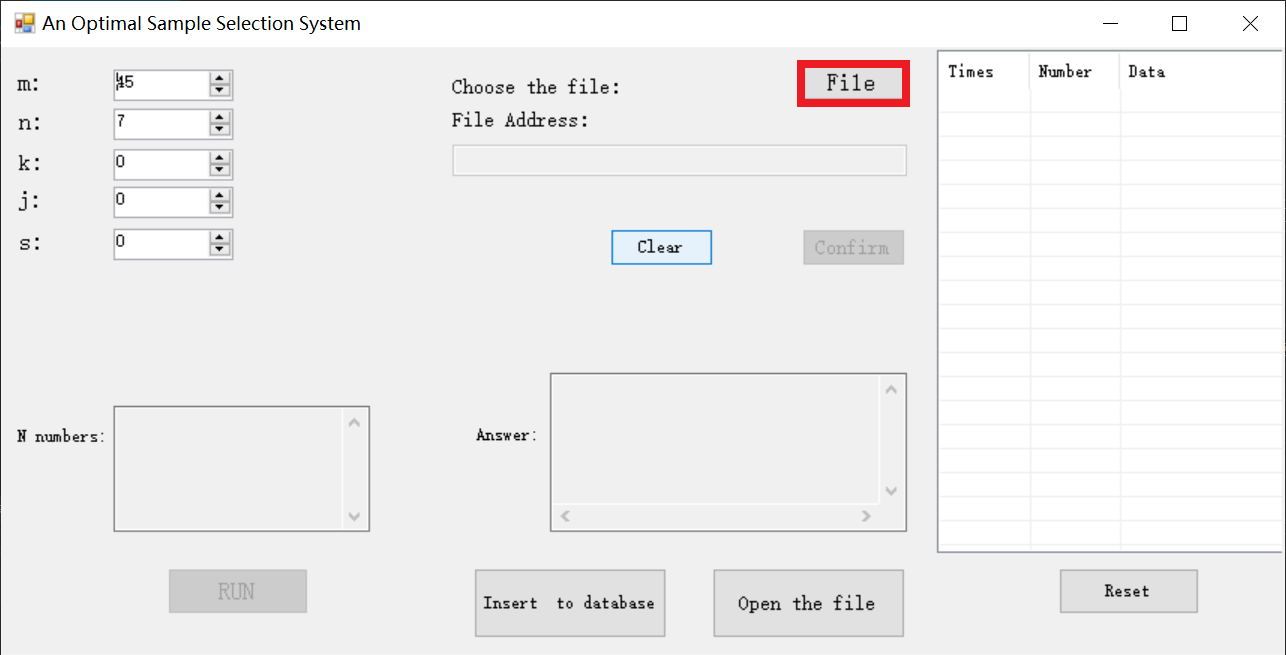
\includegraphics[width=0.75\textwidth]{images/step2.png}
	\caption{Step2}
	\label{fig:st2}
\end{figure}
\begin{figure}[!htbp]
	\centering
	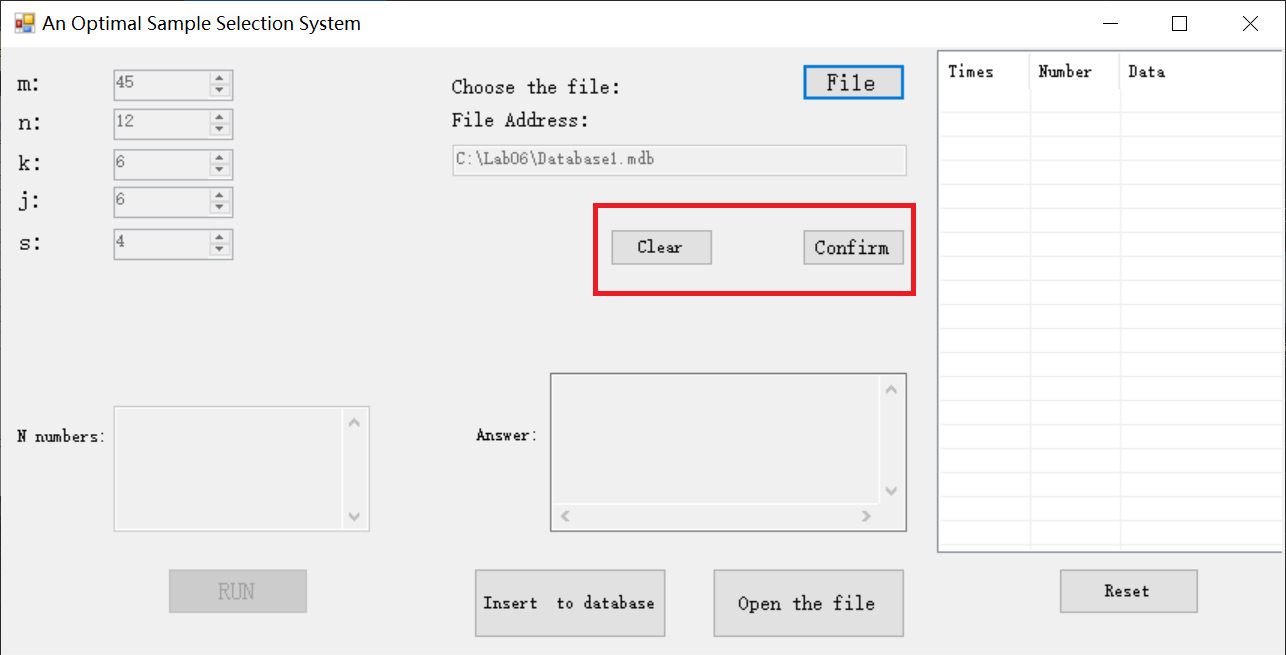
\includegraphics[width=0.75\textwidth]{images/step3.png}
	\caption{Step3}
	\label{fig:st3}
\end{figure}

\item Push the \textbf{RUN} button and the \textbf{N} number and final answer of your input will be shown 
on the surface window as Figure.\ref{fig:st4}, you can check the answer after that.
\begin{figure}[!htbp]
	\centering
	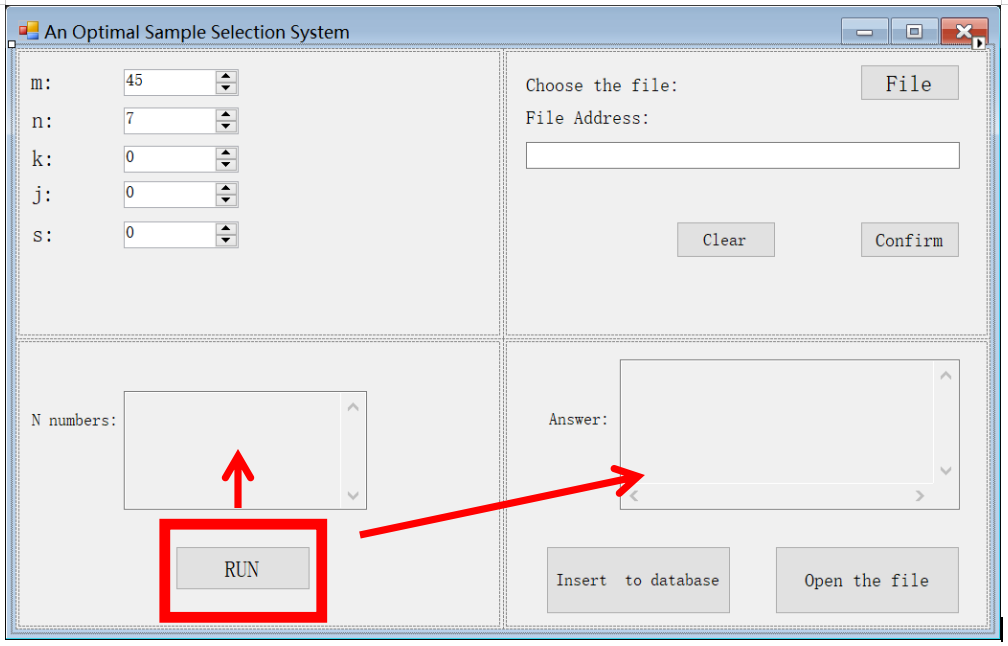
\includegraphics[width=0.75\textwidth]{images/step4.png}
	\caption{Step4}
	\label{fig:st4}
\end{figure}

\item After confirming the data is correct, use \textbf{Insert to database}(Figure.\ref{fig:st5}) 
to download the data on the DB file(\emph{\*.mdb}), and \textbf{Open the file}(Figure.\ref{fig:st6}) can open it to display the data you have calculate. 
It is also easy for you to delete or use any other operation on the data though your DB file.
\begin{figure}[!htbp]
	\centering
	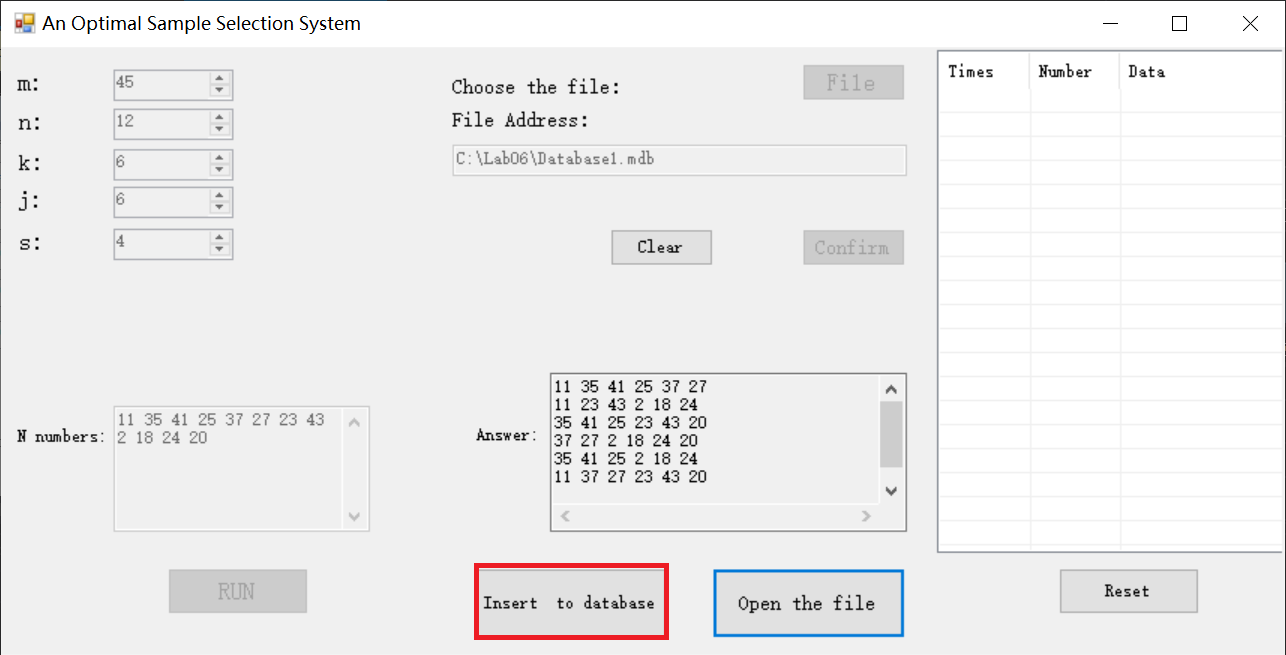
\includegraphics[width=0.75\textwidth]{images/step5.png}
	\caption{Step5}
	\label{fig:st5}
\end{figure}
\begin{figure}[!htbp]
	\centering
	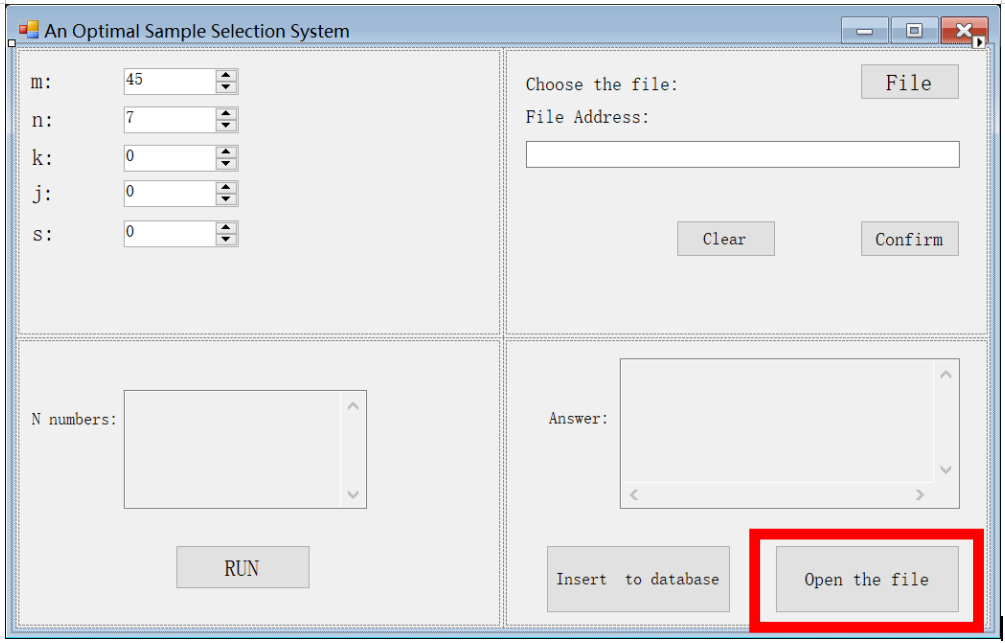
\includegraphics[width=0.75\textwidth]{images/step6.png}
	\caption{Step6}
	\label{fig:st6}
\end{figure}

\end{enumerate}